\documentclass[11pt,twoside]{book}

\usepackage[paperheight=297mm,paperwidth=210mm,width=150mm,top=30mm,bottom=30mm,bindingoffset=10mm, inner=30mm, outer=25mm]{geometry}
\usepackage[utf8]{inputenc}
\usepackage{graphicx}
\usepackage{caption}
\usepackage{subcaption}
\usepackage[nottoc]{tocbibind}
\usepackage{datetime}
\usepackage[colorlinks]{hyperref}
\usepackage{fancyhdr}
\usepackage{setspace}
\usepackage{amsmath}
\usepackage{booktabs}
\usepackage{multirow}
\usepackage{tabularx}
\usepackage{rotating}
\usepackage{titlesec}
\usepackage{tocloft}
\usepackage[acronym,nomain,nonumberlist]{glossaries}
\usepackage[table]{xcolor}
\usepackage[toc,page]{appendix}
\usepackage{pdfpages}
\usepackage{svg}
\usepackage{longtable}
\usepackage[english]{babel}
\usepackage{blindtext}

%Add acronyms if necessary
\makeglossaries


\setcounter{secnumdepth}{4}

%Copy all the images to images folder
\graphicspath{ {images/} }

%for print
%\hypersetup{citecolor=black, filecolor=black, linkcolor=black, urlcolor=black}
%for electronic
\hypersetup{citecolor=green, filecolor=black, linkcolor=blue, urlcolor=blue}

\newdateformat{monthyeardate}{\monthname[\THEMONTH] \THEYEAR}
\pagestyle{fancy}
\fancyhead{}
\fancyhead[RO,LE]{\nouppercase{\leftmark}}
\renewcommand{\headrulewidth}{0.4pt}

\renewcommand{\cftfigpresnum}{Figure\ }
\renewcommand{\cfttabpresnum}{Table\ }
\addto\captionsenglish{\renewcommand{\chaptername}{Part}}
\newcommand\blankpage{%
	\null
	\thispagestyle{empty}%
	\addtocounter{page}{-1}%
	\newpage}
\newlength{\mylenf}
\settowidth{\mylenf}{\cftfigpresnum}
\setlength{\cftfignumwidth}{\dimexpr\mylenf+2.5em}
\setlength{\cfttabnumwidth}{\dimexpr\mylenf+1.8em}
\newcolumntype{C}[1]{>{\centering\let\newline\\\arraybackslash\hspace{0pt}}m{#1}}
\definecolor{Gray}{gray}{0.95}
\newcolumntype{G}{>{\columncolor{Gray}}c}

%%%%%%%%%%%%%%%%%%%%%%%%%%
%% Document begins here %%
%%%%%%%%%%%%%%%%%%%%%%%%%%
\begin{document}

\pagenumbering{gobble}
\begin{titlepage}
    \begin{center}
        \vspace*{0cm}
        
        \begin{figure}[h]
        \begin{center}
        
\includegraphics[width=.3\columnwidth]{bbclogo.png}
        \end{center}
        \end{figure}
        \vspace*{1cm}
        
        \LARGE
        \textsc{Final NLP class Project Report}
        \vspace{1cm}
                
        \Huge
        \textbf{BBC News Analysis}
        \vspace{1.5cm}
        
        \LARGE
	 	Mahsa Ghaderan
        \vspace{1.5cm}
        
        \large 
        Supervise by
        \vspace{.5cm}
        
        \Large 
        Dr Sauleh Etemadi
        \vspace{.2cm}
        
        \setstretch{1.5}

        
     
        \vfill
        {\small \monthyeardate\today}
        
        \vspace{1cm}       
        {\Large \textbf{Department of Computer Engineering\\Iran University of Science and Technology}}
            
        \vspace*{0cm}
        
    \end{center}
\end{titlepage} %\pagenumbering{gobble} if we need to remove page numbering

\blankpage
\setstretch{1.0}
\clearpage
\newpage
\tableofcontents
\newpage
\listoffigures
\newpage
\listoftables
\glsaddall
\printglossary[type=\acronymtype,title=List of Acronyms]
\addcontentsline{toc}{chapter}{List of Acronyms}

\setstretch{1.0}
\chapter{Word2Vec}
\pagenumbering{arabic} %Start Arabic page numbering
\setstretch{1.5}
\label{chapter:word2vec}


In this part I used assignment2 from cs224n, 2021 Stanford NLP course as my base code. Different Word2Vec models are trained for each label which exist in BBC data set. Headline is concatenated with body of each news for as input text for the model. Each models trains for 40000 iteration. It took about 5 hours for each label. Wights of models are saved is "models/word2vec" directory. Most 30 repeated words are chosen from each label. Images - , - , - and - shows distribution of each model on a 2D map. 


\section{Iran News}
After training word2vec model we exoect to see words with same meaning appear near to ech other and words with far meaning and context place far from others on each map.
\begin{figure}[h]
	\centering
	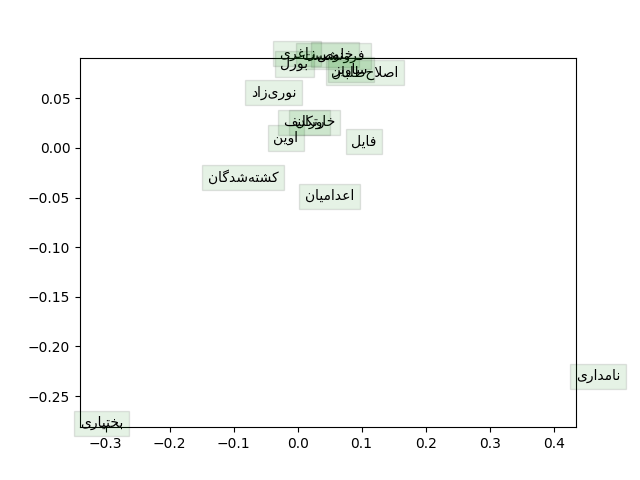
\includegraphics[width=10cm]{../reports/word2vec/word_vectors_ايران.png}
	\caption{Sub-words vocab example}
	\label{fig:word2veciran}
\end{figure}


\section{Art News}
\begin{figure}[h]
	\centering
	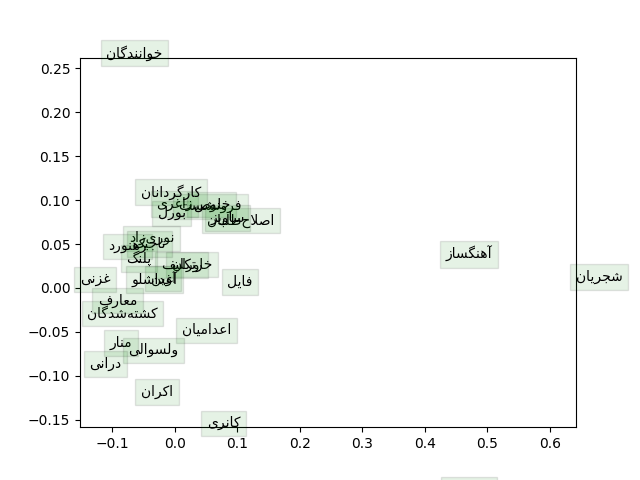
\includegraphics[width=10cm]{../reports/word2vec/word_vectors_هنر.png}
	\caption{Sub-words vocab example}
	\label{fig:word2vecart}
\end{figure}


\section{Sport News}
\begin{figure}[h]
	\centering
	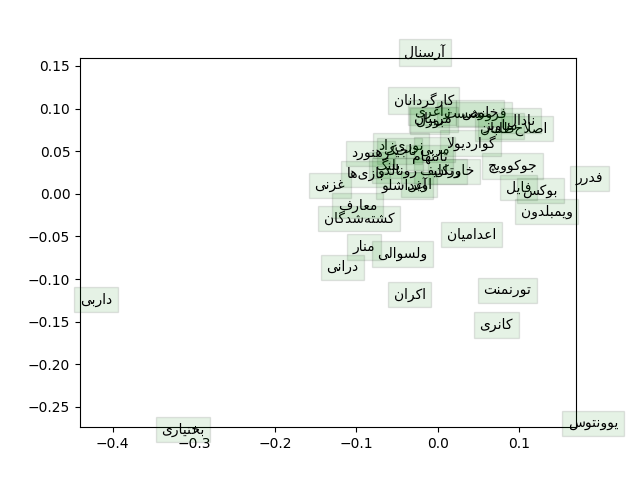
\includegraphics[width=10cm]{../reports/word2vec/word_vectors_ورزش.png}
	\caption{Sub-words vocab example}
	\label{fig:word2vecsport}
\end{figure}


\section{Economic News}
In map \ref{fig:word2vececon} words in car and it's factory are gathered in the left part of the image.
\begin{figure}[h]
	\centering
	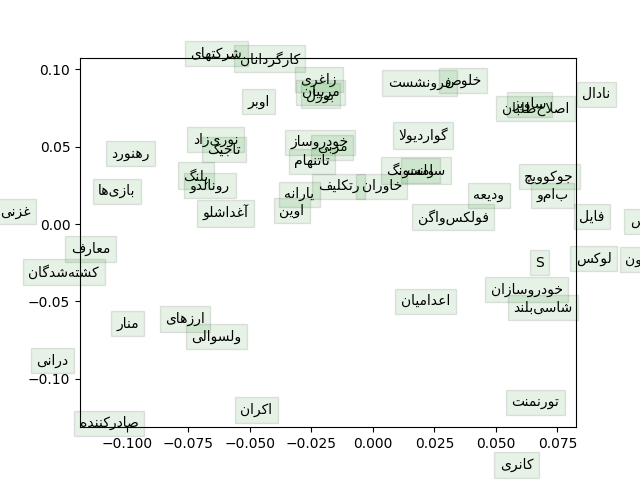
\includegraphics[width=10cm]{../reports/word2vec/word_vectors_اقتصاد.png}
	\caption{Sub-words vocab example}
	\label{fig:word2vececon}
\end{figure}

\section{Science News}
At map \ref{fig:word2vecsience} words are overlapped and it's not easy to distinguish them. Equivalent of two words Astronauts and UFO persia are in same context and located almost near to each other and far from others. Two other words are composer and name of a popular Iranian singer, Shajarian, are placed next to each other.
\begin{figure}[h]
	\centering
	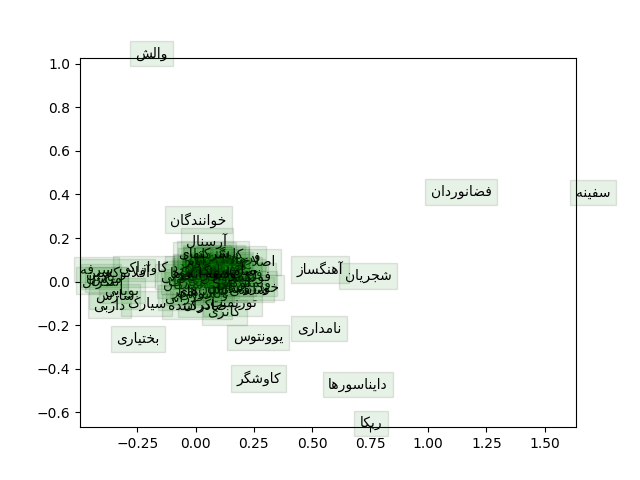
\includegraphics[width=10cm]{../reports/word2vec/word_vectors_دانش.png}
	\caption{Sub-words vocab example}
	\label{fig:word2vecsience}
\end{figure}


\setstretch{1.0}
\chapter{Tokeniation}
\setstretch{1.5}
\label{chapter:literature}

SentencePiece is an unsupervised text tokenizer and detokenizer python project, which mainly used for text generation tass.This part ia mainly based on this packet. It use a model to train what tokens are best to tokenizing a given corpus. In this part 2 different methods of tokenization in implemented. First is tokenizing words and sub-words, in this methods model looking for most repeated words and sub-words and even letter. As a result we can see almost every word in final version of chosen tokens. On the contrary the second method is just tokenizing words, this models looking for most repeated words. 
\newline
Until this part entire headline and body of each news are both covered in the corpus but from this part English values are removed from corpus so tokenization and language generation will focus on Persian. 
\newline
The corpus is shuffled 5 times and separated to train and test data. Also tokenization is applied on 4 different vocab size due to possible SentencePiece size and performance of output model is evaluated against these vocab size. In the following section, we discuss about effects of vocab size from very small value increasing to a large value.
\newline

\section{Sub-word Level}
At first i train tokenizer model on sub-words. It means model not only pays attention to words, but also pays attention to sub-words during training time. 

When the vocab size is 1000, it is too small for such a corpus and due to model type, model focuce on smaller sub-words rather than meaning full words. In final choosed-vocab, almost every character in source language exists. So when we tokenize a text there woudln't be any <unk> token and most words break into sub-words. 
\newline
As vocab size increases model learns more complicated sub-words and less meaning-less characters and sub-words. Bot the negative point is as the vocab size increases it would be harder for models to learn task and the positive point is more context will be save after tokenization.

Another point is SentencePiece can discriminate between statrting token and not starting token and ending token of a word in this mode. As we can see in \ref{fig:word2vecsubword} the are different form of one token.

\begin{figure}[h]
	\centering
	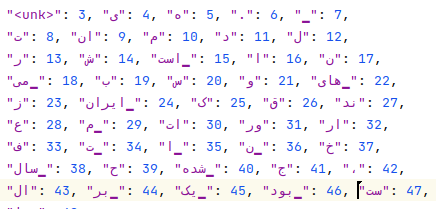
\includegraphics[width=10cm]{images/word2vec_subwordtockens.png}
	\caption{Sub-words vocab example}
	\label{fig:word2vecsubword}
\end{figure}


\section{Word Level}
In this part, i used word level tokenization, in this experience there exist <unk> token due to vocab size and model dealing with choosing best token in order to minimize <unk> token in unseen text. 
\newline
Same as previous experiment, data-set is divided into train and test set and 5 different shuffled corpus is saved, this help us to have a better evaluation on each vocab size. Four different vocab size is defined as follow: 1000, 5000, 10000, 15000. Number of <unk> token and percent of that over each corpus and vocab is reported in "report/tokenization" directory and each model and output on test set is saved in "src/tokenization/working-dir/words-out". percent of each vocab size is presented in table \ref{tbl:token-unk}.

\begin{center}
	\centering
	\begin{tabular}{|c|| c|c|c|c|c||G |} 
		\hline 
		& \multicolumn{6}{c|}{word-level} \\
		\hline
		corpus & 1 & 2 & 3 & 4 & 5 & AVG\\	
		\hline
		1000   & 0.44 & 0.44 & 0.44 & 0.43 & 0.44 & 0.44\\
		5000   & 0.20 & 0.20 & 0.20 & 0.20 & 0.20 & 0.21\\
		10000  & 0.14 & 0.14 & 0.14 & 0.14 & 0.15 & 0.15\\
		15000  & 0.12 & 0.12 & 0.12 & 0.12 & 0.14 & 0.13\\
		\hline 
	\end{tabular}
	\label{tbl:token-unk}
\end{center}

As it is illustrated in table \ref{tbl:token-unk}, number of <unk> token increase by vocab size reduction. the fewer <unk> token, the fewer information loss. On the other the larger vocab size leads into more amount of computaion for future task. As we saw it is a trade of between these to parameters, in my opinion best vocab size due to this corpus is \textbf{10000}. It has reasonable <unk> token and it may need less computation rather than 15000 vocab size.
\newline
After tokenizing corpus in word level, we can see <unk> tokens besides tokens which exist in vocabulary. In this project <unk> token id is equal to 3. Many <unk> token can be seen in tokenized validation set (Figure \ref{fig:unkrep}).

\begin{figure}[h]
	\centering
	
\includegraphics[width=15cm]{images/unkrep.png}
	\caption{Tokenized Corpus}
	\label{fig:unkrep}
\end{figure}



\chapter{Language Model}
\setstretch{1.5}
\label{chapter:experiments}
 
Language model neural network artichecture is adopt from \href{https://github.com/pytorch/examples/tree/master/word_language_model}{pytorch/examples} project. Tokenizer codes and models are replaced with Part 2 and vocab for Language Modeling is construct in part 2. In this part the corpus is divided into three part, train set, dev set and test set. LanguageModel is trained on each label separately to evaluate capability of each model to generate specific news. Models are saved in "models/lm" directory. 
Models are trained on GTX1070 GPU. training process is 10 time faster than CPU. 
\section{LSTM}
Use LSTM architecture(Figure \ref{fig:mylstm}) for language model. Best perplexity recorded is 47 on "Science" label. Each epoch last about 0.36 second, perplexity method starts from 60 and it is 43 on validation data on last epoch.\ref{fig:lstm_education}

\begin{figure}
	\centering
	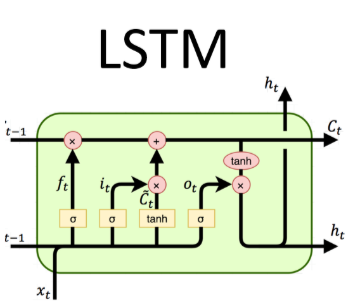
\includegraphics[width=10cm]{images/lstm.png}
	\caption{LSTM Architecture}
	\label{fig:mylstm}
	
\end{figure}

\begin{figure}
	\centering
	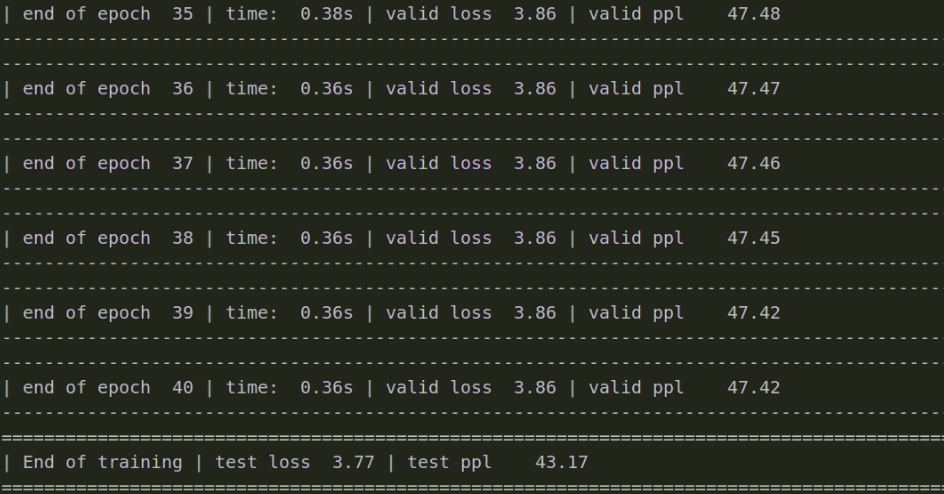
\includegraphics[width=10cm]{images/lstm_danesh.png}
	\caption{Perplexity LSTM language model, label = Science}
	\label{fig:lstm_education}
\end{figure}

In this trial, there are many <unk> token in output generated text. But generated sentences are in "Science" context.\ref{fig:gru_education_out}
\begin{figure}
	\centering
	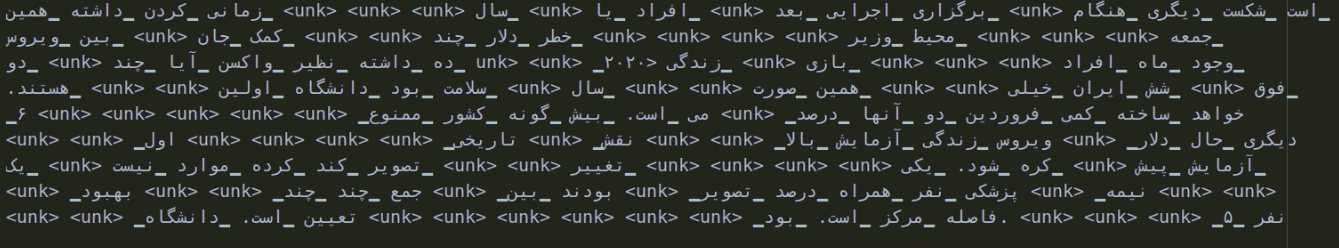
\includegraphics[width=15cm]{images/lstm_danesh_out.png}
	\caption{Generated Text LSTM language model, label = Science}
	\label{fig:gru_education_out}
\end{figure}

\section{GRU}

Use GRU architecture (Figure \ref{fig:mygru}) for language model. Few Last epochs and output is illustrated in figure \ref{fig:gru_education}. LSTM and GRU have similar learning power as a evidence perplexity of GRU model on test set is 43, when label is "Science", same as LSTM. Each epoch last about 0.33 second as expected GRU model is faster, compare to LSTM model. 


\begin{figure}
	\centering
	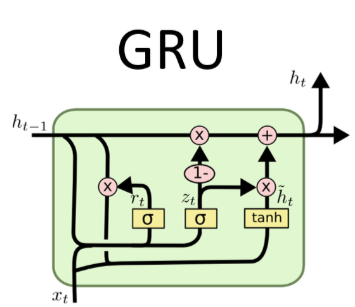
\includegraphics[width=10cm]{images/gru.png}
	\caption{GRU Architecture}
	\label{fig:mygru}
	
\end{figure}

\begin{figure}
	\centering
	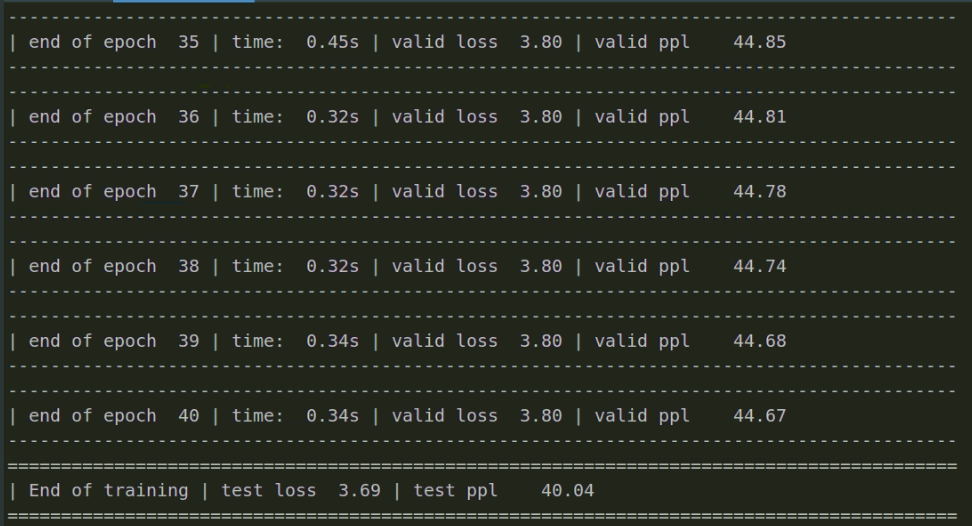
\includegraphics[width=10cm]{images/gru_danesh.png}
	\caption{Perplexity GRU language model, label = Science}
	\label{fig:gru_education}
\end{figure}

In this trial, again there are many <unk> token in output generated text. Generated sentences are in "Education" context.\ref{fig:gru_edu_out}

\begin{figure}
	\centering
	
\includegraphics[width=15cm]{images/gru_danesh_out.png}
	\caption{Generated Text GRU language model, label = Science}
	\label{fig:gru_edu_out}
\end{figure}

\section{Transformer}
In last trial Transformer architecture is used for language model. Few Last epochs and output is illustrated in figure \ref{fig:transformer_edu}. LSTM and GRU both have almost similar learning power, but with transformer architecture it is possible to access better results. As shown in Figure \ref{fig:transformer_edu_out} test perplexity is 37.41, when label is "Science" which is 3 score better than previous models. Each epoch last longer than previous models and it is about 0.40 second.
 
\begin{figure}
	\centering
	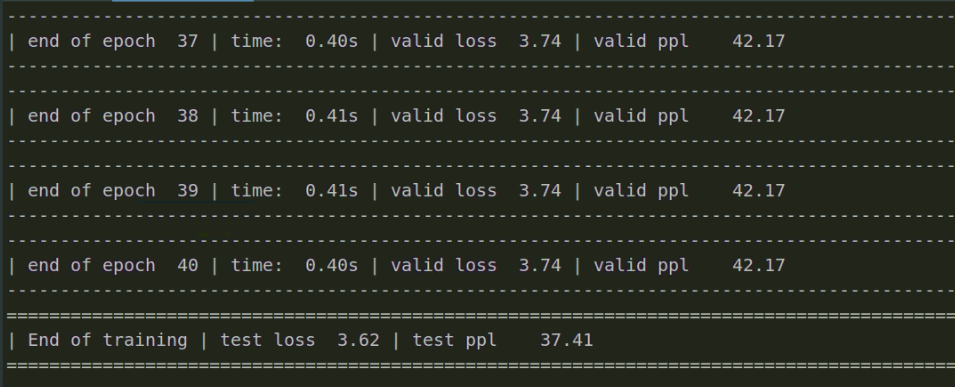
\includegraphics[width=10cm]{images/transformer_danesh.png}
	\caption{Perplexity Transformer language model, label = Science}
	\label{fig:transformer_edu}
\end{figure}

In this trial generated text is shown in \ref{fig:transformer_edu_out}. Number of <unk> token is decreased and there are more meaningful sentences. Generated sentences are in "Science" context.
\begin{figure}
	\centering
	
\includegraphics[width=15cm]{images/transformer_danesh_out.png}
	\caption{Generated Text Transformer language model, label = Science}
	\label{fig:transformer_edu_out}
\end{figure}

Run "bash run.sh 4" to train all three types of language models. Models will save in "models/lm" directory. Then run "bash run.sh 41" in order to generate text for each label. For each model generated text will save in corresponding file in "reports/lm" directory.

\section{Temperature}
Different temperature can be used when generating text. If set temperature low, generated text will be more general, as a result number of <unk> token will increase. On the other hand by setting higher value for temperature model diversity increases. For this project 1 is best choice for temperature parameter.
    
\section{Final Outputs} 
In this section output of each label on trained transformer-based language model is represented. 
\subsection{Iran}
Iran news is largest corpus in this dataset. We can see more meaningful sentences and less <unk> tokens. Generated sentences seems link Iran news and generated-words illustrated in Figure \ref{fig:iran} are related to the context. 
\begin{figure}
	\centering
	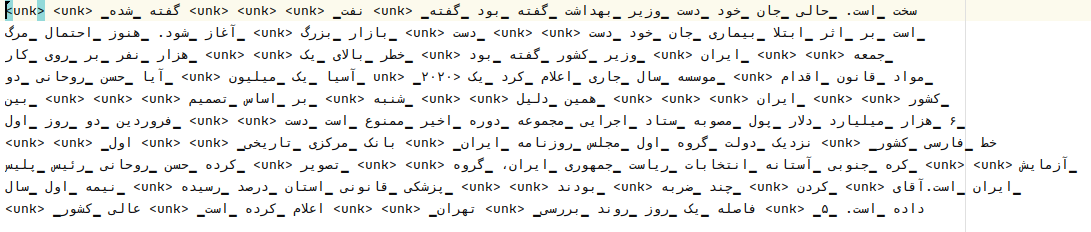
\includegraphics[width=15cm]{images/iran.png}
	\caption{Generated Text Transformer language model, label = Iran}
	\label{fig:iran}
\end{figure}

\subsection{Art}
Longest n-gram in generated text without any <unk> token is placed on second line, which n is equal to 10(Figure \ref{fig:art}). This sequence of words is not meaningful enough, but seems fluent. 
\begin{figure}
	\centering
	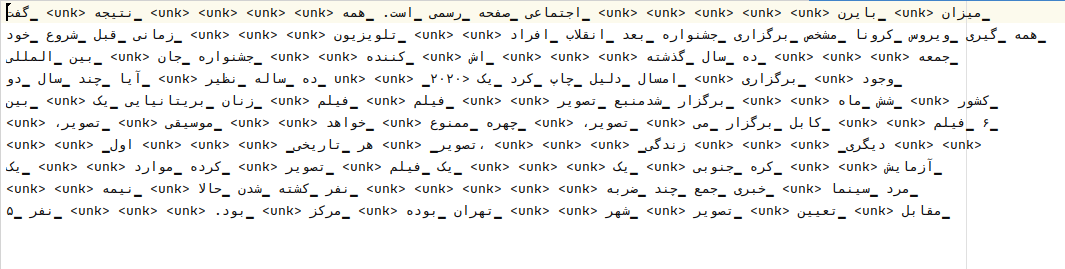
\includegraphics[width=15cm]{images/art.png}
	\caption{Generated Text Transformer language model, label = Art}
	\label{fig:art}
\end{figure}
\subsection{Science}
In this section there are many <unk> tokens due lack of data in Science class. Longest sequence of words is 4-grams and used words are more general than other sections.
\begin{figure}
	\centering
	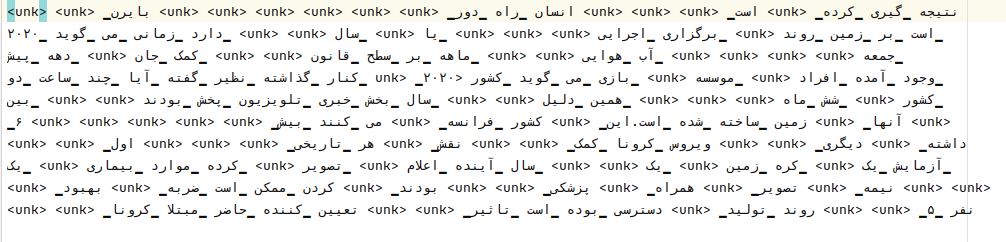
\includegraphics[width=15cm]{images/science.png}
	\caption{Generated Text Transformer language model, label = Science}
	\label{fig:science}
\end{figure}
\subsection{Economic}
In Economic class generated field as it is shown in figure \ref{fig:economic} most at least 6-grams are construct of meaningful sequences of words and they sounds same as economic news. We can see many 8-grams without any <unk> token in this section. 
\begin{figure}
	\centering
	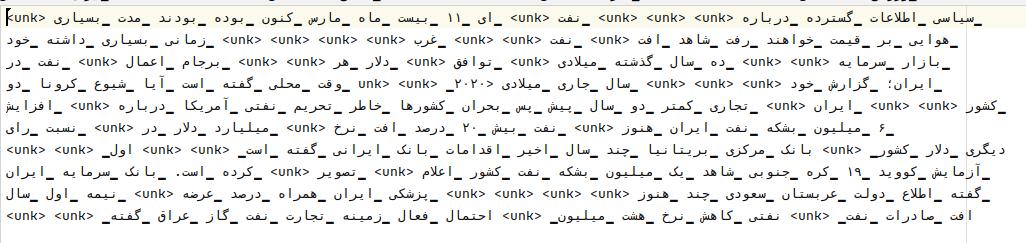
\includegraphics[width=15cm]{images/economic.png}
	\caption{Generated Text Transformer language model, label = Economic}
	\label{fig:economic}
\end{figure}
\subsection{Sport}
In this class, generated text includes of variety of meaningful n-grams without any <unk> token. It is interesting that fluent and meaning 9-garms sequence of words is constructed.(Line 4, Figure \ref{fig:sport})
\begin{figure}
	\centering
	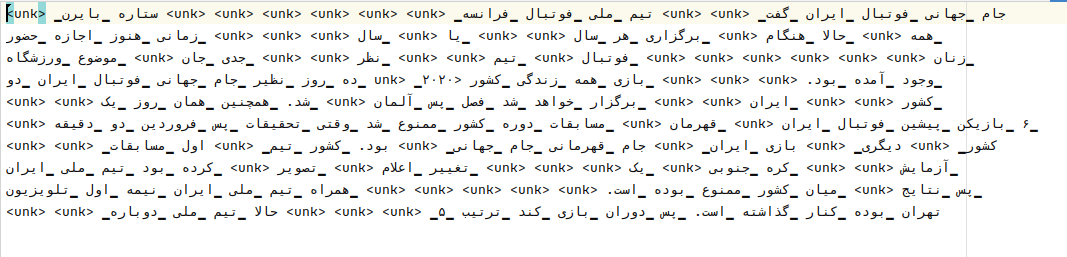
\includegraphics[width=15cm]{images/sport.png}
	\caption{Generated Text Transformer language model, label = Sport}
	\label{fig:sport}
\end{figure}


\chapter{Finetuning}
\setstretch{1.5}
\label{chapter:discussion}

In this part ParsBert V3 is used as pre-trained Bert model. PyTorch version is used. Due to hardware limitation train batch size is set to 4 and evaluation batch size is set to 8.
Model save into reports directory every 500 iteration. In first experiments whole data is used to fine-tune BERT model. As a result BERT is fine-tuned on news data set. Next step is to extract on layer before last one as embedding(a representation for each word) and replace task 4 embedding part with this model. 
Tokenization result for one sample is represented is Figure \ref{fig:fine}.

\begin{figure}
	\centering
	
\includegraphics[width=15cm]{images/tkn.png}
	\caption{Tokenization based on BERT model for an input sentences.}
	\label{fig:fine}
\end{figure}

\end{document}
